\documentclass[11pt]{article}
% \usepackage[margin=1in]{geometry}
\usepackage[top=1in, bottom=1in, left=.5in, right=.5in]{geometry} % see geometry.pdf on how to lay out the page. There's lots.
\usepackage{amsmath,amsthm,amssymb}

% Ignore spaces in filenames
\usepackage[space]{grffile}

\usepackage[T1]{fontenc}
\usepackage{bigfoot} % to allow verbatim in footnote
\usepackage[numbered,framed]{matlab-prettifier}
\usepackage{filecontents}
\usepackage{graphicx}
\usepackage[normalem]{ulem}

\let\ph\mlplaceholder % shorter macro
\lstMakeShortInline"

\lstset{
  style              = Matlab-editor,
  basicstyle         = \mlttfamily,
  escapechar         = ",
  mlshowsectionrules = true,
}

\title{MAE 275 - Midterm}
\author{John Karasinski}
\date{May 22, 2015}

\begin{document}
\maketitle

\section{Defining the System}
The state-space system can be defined,
\begin{equation*}
\begin{split}
\dot{\vec{x}} = A\vec{x} + B\vec{u} \\
      \vec{y} = C\vec{x} + D\vec{u}
\end{split}
\end{equation*}

\noindent where the linearized longitudinal aircraft equations of motion can be expressed in state space form.

$$
\vec{x}= \left[ \begin{array}{c}        u \\ w        \\ q   \\ \theta \\       h \end{array} \right], \qquad
\vec{u}= \left[ \begin{array}{c} \delta_e \\ \delta_T \\ u_g                      \end{array} \right], \qquad
\vec{y}= \left[ \begin{array}{c}        u \\ \alpha   \\ h   \\ \dot{h} \\ \theta \end{array} \right] 
$$

\begin{equation*}
A =
\begin{bmatrix}
    X_u & X_w & 0 & -g \cos(\theta_0) & 0 \\
    \dfrac{Z_u}{1-Z_{\dot{w}}} & \dfrac{Z_w}{1-Z_{\dot{w}}} & \dfrac{Z_q + u_0}{1-Z_{\dot{w}}} & -\dfrac{g\sin \theta_0}{1-Z_{\dot{w}}} & 0 \\
    M_u + \dfrac{M_{\dot{w}} Z_u}{1-Z_{\dot{w}}} & M_w + \dfrac{M_{\dot{w}} Z_w}{1-Z_{\dot{w}}} & M_q + \dfrac{M_{\dot{w}} (Z_q + u_0)}{1-Z_{\dot{w}}} & -\dfrac{M_{\dot{w}} g\sin \theta_0}{1-Z_{\dot{w}}} & 0 \\
    0 & 0 & 1 & 0 & 0 \\
    0 & -1 & 0 & u_0 & 0
\end{bmatrix}
\end{equation*}

\noindent Relevant B, C, and D matrices can also be formed
\begin{equation*}
B =
\begin{bmatrix}
    X_{\delta_e}                                                   & X_{\delta_T}                                                   & -X_u                                          \\
    \dfrac{Z_{\delta_e}}{1-Z_{\dot{w}}}                            & \dfrac{Z_{\delta_T}}{1-Z_{\dot{w}}}                            & \dfrac{-Z_u}{1-Z_{\dot{w}}}                   \\
    M_{\delta_e} + \dfrac{M_{\dot{w}} Z_{\delta_e}}{1-Z_{\dot{w}}} & M_{\delta_T} + \dfrac{M_{\dot{w}} Z_{\delta_T}}{1-Z_{\dot{w}}} & -M_u - \dfrac{M_{\dot{w}} Z_u}{1-Z_{\dot{w}}} \\
    0   &  0   &  0 \\
    0   &  0   &  0 \\
\end{bmatrix}
\end{equation*}

\begin{equation*}
C =
\begin{bmatrix}
    1 &          0     & 0 & 0   & 0\\
    0 & \dfrac{1}{u_0} & 0 & 0   & 0\\
    0 &          0     & 0 & 0   & 1\\
    0 &         -1     & 0 & u_0 & 0\\
    0 &          0     & 0 & 1   & 0\\
\end{bmatrix},
\qquad
D =
\begin{bmatrix}
    0 & 0 & 0 \\
    0 & 0 & 0 \\
    0 & 0 & 0 \\
    0 & 0 & 0 \\
    0 & 0 & 0 \\
\end{bmatrix}
\end{equation*}

\clearpage
\noindent Using the longitudinal equations of motion for C-5A for level flight ($u_0=246$ ft/s) at sea level, the resultant system is

$$
\dot{\vec{x}} = \left[ \begin{array}{ccccc}
  -0.0214              &  +0.0957             &    0      &  -32.2 & 0 \\
   -0.231              &  -0.634              & +246      &    0   & 0 \\
   +1.964\times10^{-4} &  -8.895\times10^{-4} &   -0.8275 &    0   & 0 \\
    0                  &   0                  &    1      &    0   & 0 \\
    0                  &  -1                  &    0      & +246   & 0 \end{array} \right]
\vec{x} + \left[\begin{array}{ccc}
      +0.45            & +0.554\times10^{-4}  & +0.0214                \\ 
      -9.53            & -0.193\times10^{-5}  & +0.231                 \\
    -0.6795            & +1.4571\times10^{-7} & -1.9642\times10^{-4}   \\ 
          0            &  0                   &  0                     \\ 
          0            &  0                   &  0 \end{array}\right] \vec{u}  
$$

$$
\vec{y} = \left[ \begin{array}{ccccc}
         1 &   0      &   0   &    0   &  0 \\
         0 &   0.0041 &   0   &    0   &  0 \\
         0 &   0      &   0   &    0   &  1 \\
         0 &  -1      &   0   &  246   &  0 \\
         0 &   0      &   0   &    1   &  0 \end{array} \right]
\vec{x}+\left[\begin{array}{ccc}
         0 &   0      & 0 \\ 
         0 &   0      & 0 \\
         0 &   0      & 0 \\
         0 &   0      & 0 \\
         0 &   0      & 0 \end{array}\right]\vec{u}
$$
         
\vspace{25pt}
The loops are sequentially closed in the order: $\theta\rightarrow\delta_e$, $u\rightarrow\delta_T$, $\dot{h}\rightarrow\theta_e$.
The following pages lists the linearized transfer functions used to design the compensators, along with the transfer function of each compensator.
The gain and phase margins and bandwidth are also listed for the compensated loop.

\begin{figure}[b!]
\begin{center}
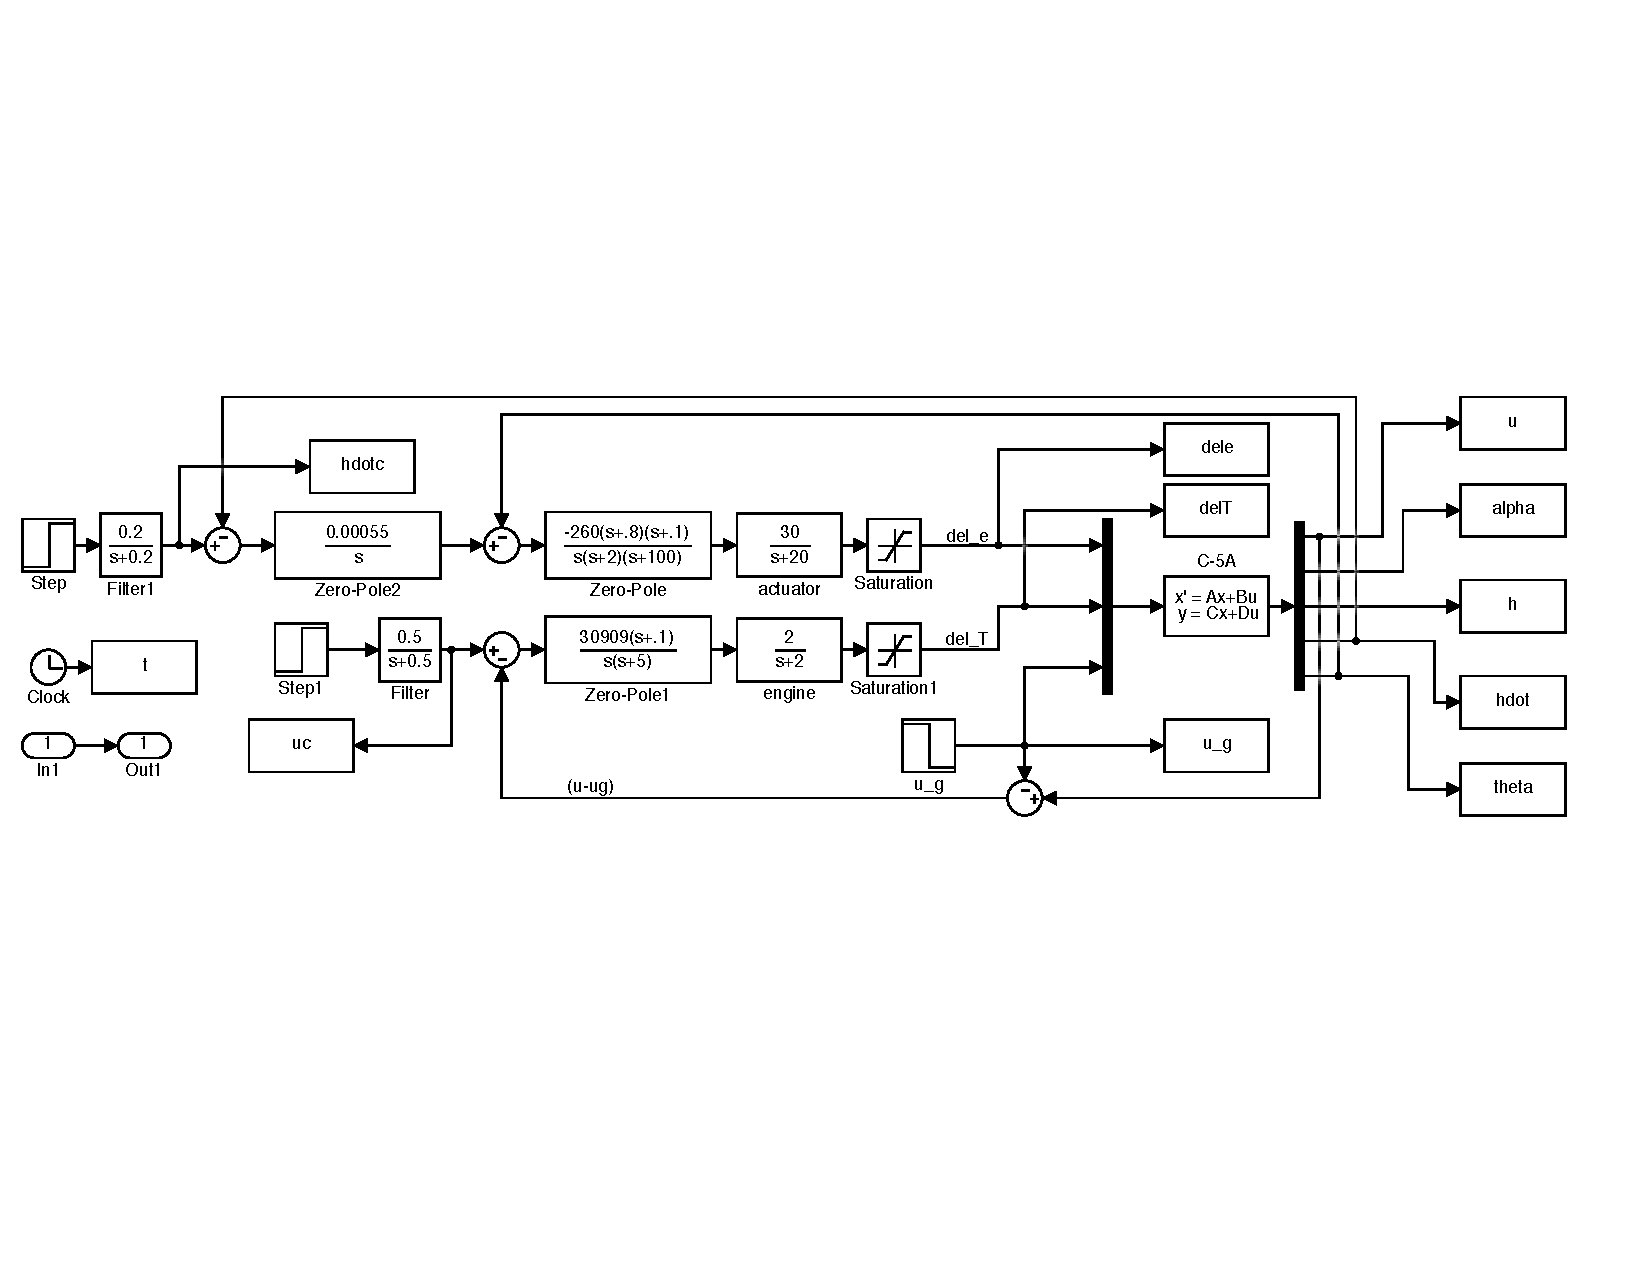
\includegraphics[width=1\textwidth]{figures/final_simulink}
\caption{Final Simulink Model}
\end{center}
\end{figure}

\clearpage
\section{Compensators}

\begin{gather*}
\frac{\theta}{\delta_e}=\frac{-20.387 (s+0.5819) (s+0.06093)}{(s+20) (s^2 + 0.02027s + 0.01411) (s^2 + 1.463s + 0.7531)} \\
\\
\boxed{Gc_{\theta} = -260 \times \frac{(s+0.8)(s+0.1)}{s(s+2)(s+100)}} \\
\\
G_m=22.4\,\mathrm{dB\,\, at\,} 5.64 \,\mathrm{rad/s}  \\
P_m=57.9^{\circ}\, \mathrm{at}\, 1.18 \,\mathrm{rad/s} \\
\omega_{BW}=1.98\, \mathrm{rad/s}\,\mathrm{\,(3 dB\, criterion)}\\
\end{gather*}

\begin{figure}[b!]
\begin{center}
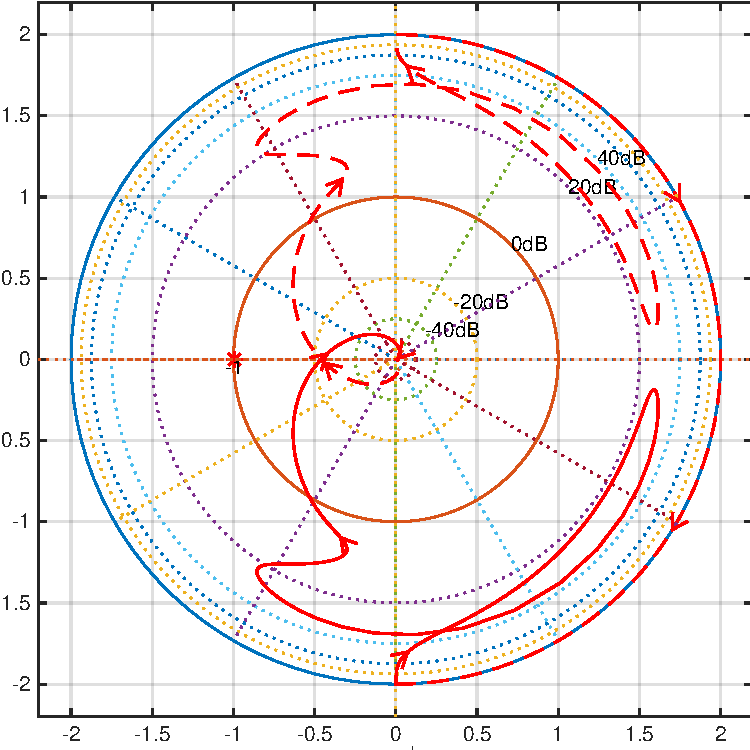
\includegraphics[height=.4\textheight]{figures/nyquist_theta}
\caption{Nyquist Diagram for $\dfrac{\theta}{\delta_e}$}
\end{center}
\end{figure}

\begin{figure}[h!]
\begin{center}
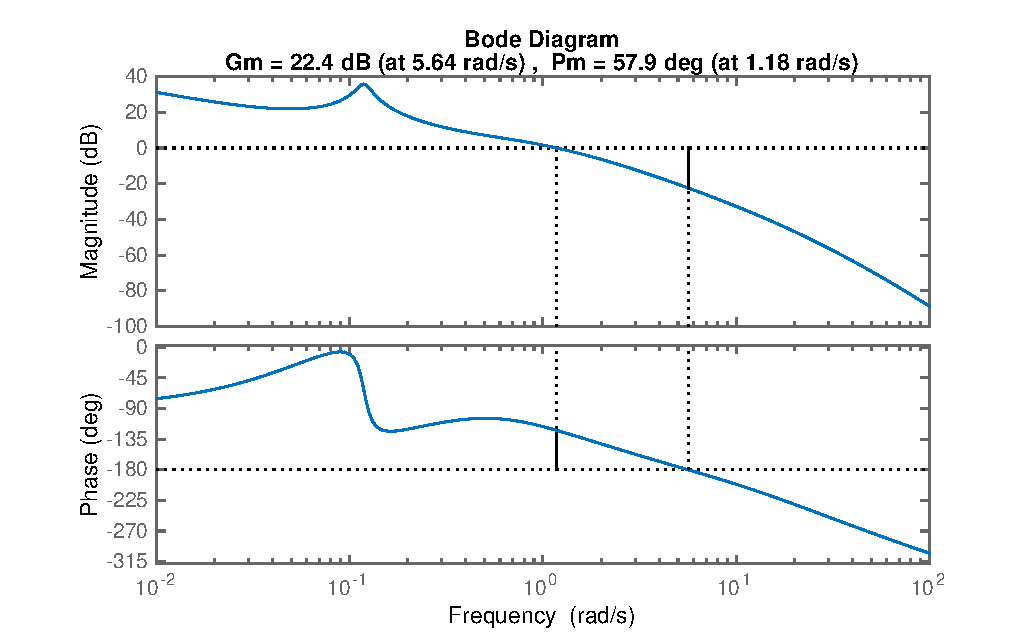
\includegraphics[height=.4\textheight]{figures/open_comp_theta}
\caption{Open-loop Compensated Bode Diagram for $\dfrac{\theta}{\delta_e}$}
\end{center}
\end{figure}

\begin{figure}[h!]
\begin{center}
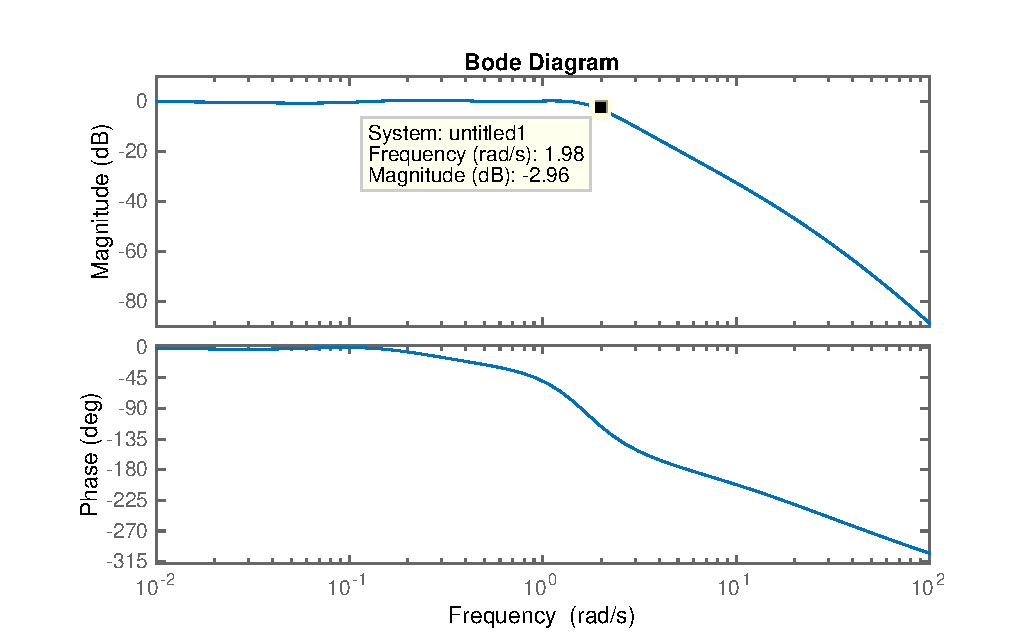
\includegraphics[height=.4\textheight]{figures/close_comp_theta}
\caption{Close-loop Compensated Bode Diagram for $\dfrac{\theta}{\delta_e}$}
\end{center}
\end{figure}

\begin{gather*}
\frac{u}{\delta_T}=\frac{0.0001108 (s+1.093) (s+0.3076) (s+0.1381) (s^2 + 1.745s + 2.785)}{(s+2) (s+1.078) (s+0.0452) (s^2 + 0.4706s + 0.05552) (s^2 + 1.716s + 2.754)} \\
\\
\boxed{Gc_{\dot{h}} = 30909 \times \frac{(s+0.1)}{s(s+5)}} \\
\\
G_m=25.7\,\mathrm{dB\,\, at\,} 3.08 \,\mathrm{rad/s}  \\
P_m=72.3^{\circ}\, \mathrm{at}\, 0.351 \,\mathrm{rad/s} \\
\omega_{BW}=0.499\, \mathrm{rad/s}\,\mathrm{\,(3 dB\, criterion)}\\
\end{gather*}

\begin{figure}[b!]
\begin{center}
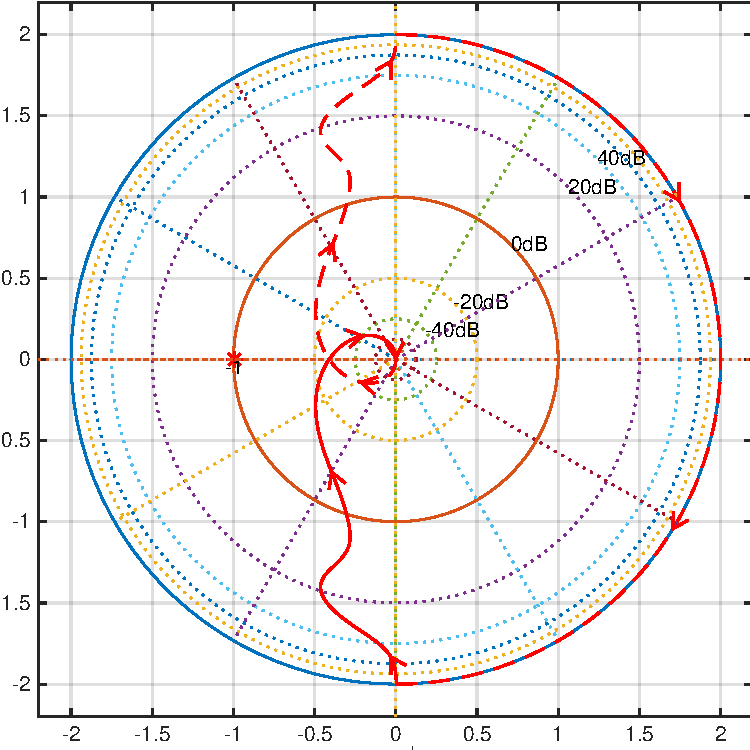
\includegraphics[height=.4\textheight]{figures/nyquist_u}
\caption{Nyquist Diagram for $\dfrac{\theta}{\delta_e}$}
\end{center}
\end{figure}

\begin{figure}[h!]
\begin{center}
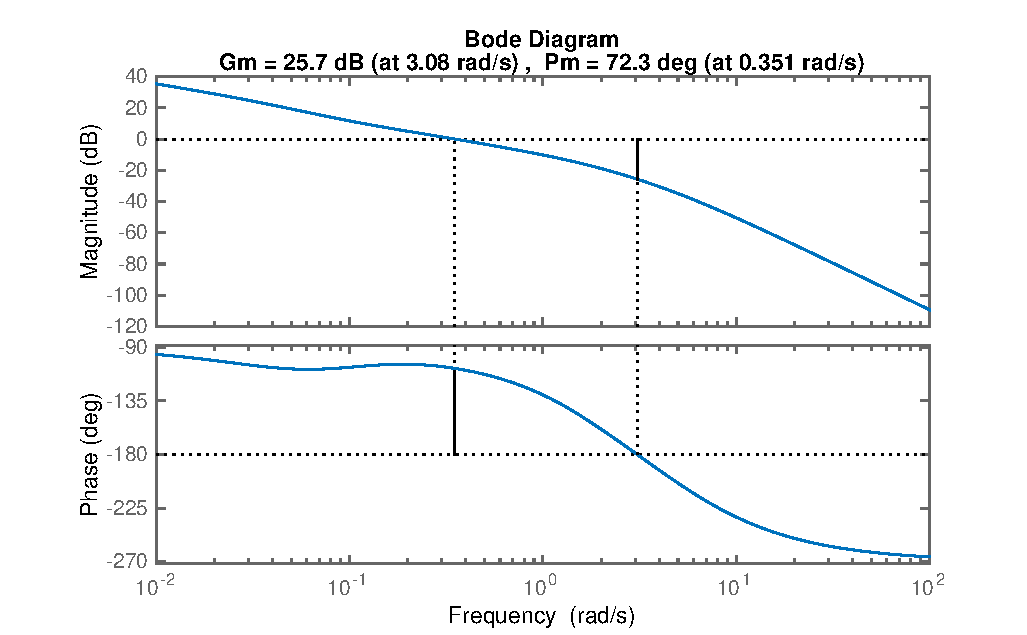
\includegraphics[height=.4\textheight]{figures/open_comp_u}
\caption{Open-loop Compensated Bode Diagram for $\dfrac{u}{\delta_T}$}
\end{center}
\end{figure}

\begin{figure}[h!]
\begin{center}
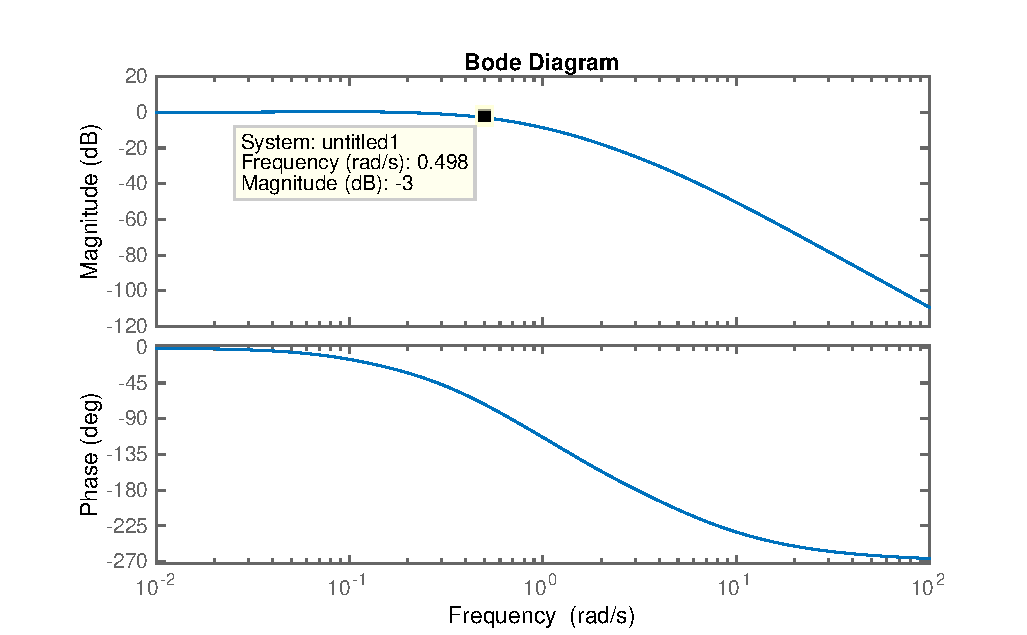
\includegraphics[height=.4\textheight]{figures/close_comp_u}
\caption{Close-loop Compensated Bode Diagram for $\dfrac{u}{\delta_T}$}
\end{center}
\end{figure}

\begin{gather*}
\frac{\dot{h}}{\theta_e}=\frac{-74334 (s+3.752) (s+1.35) (s+0.8) (s+0.2827) (s+0.1736) (s+0.1) (s-2.901)}{(s+99.99) (s+20.18) (s+1.371) (s+0.9979) (s^2 + 0.2143s + 0.01295) (s^2 + 0.8171s + 0.1759) (s^2 + 1.707s + 2.74)} \\
\\
\boxed{Gc_{u} = 0.00055 \times \frac{1}{s}} \\
\\
G_m=19.8\,\mathrm{dB\,\, at\,} 0.785 \,\mathrm{rad/s}  \\
P_m=68.1^{\circ}\, \mathrm{at}\, 0.132 \,\mathrm{rad/s} \\
\omega_{BW}=0.202\, \mathrm{rad/s}\,\mathrm{\,(3 dB\, criterion)}\\
\end{gather*}

\begin{figure}[b!]
\begin{center}
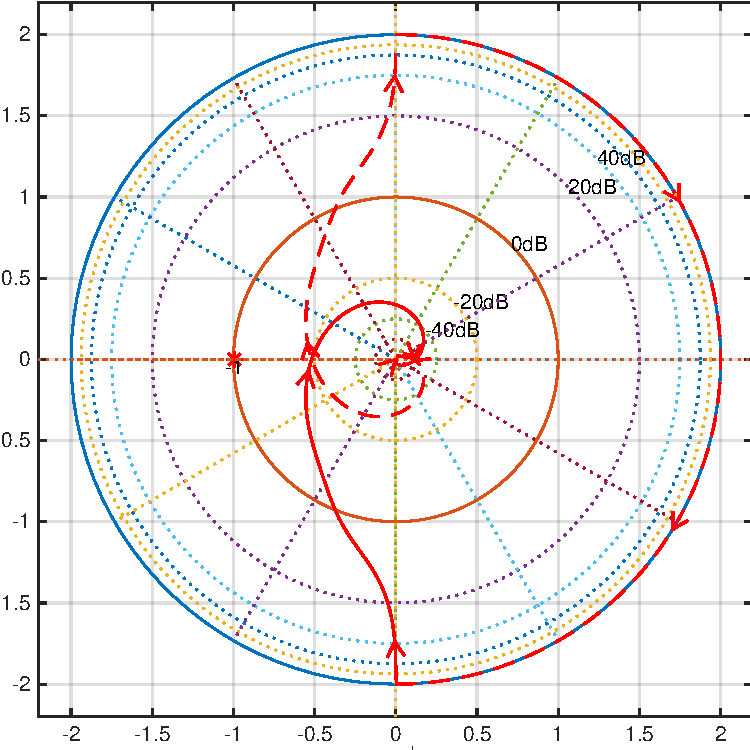
\includegraphics[height=.4\textheight]{figures/nyquist_hdot}
\caption{Nyquist Diagram for $\dfrac{\theta}{\delta_e}$}
\end{center}
\end{figure}

\begin{figure}[h!]
\begin{center}
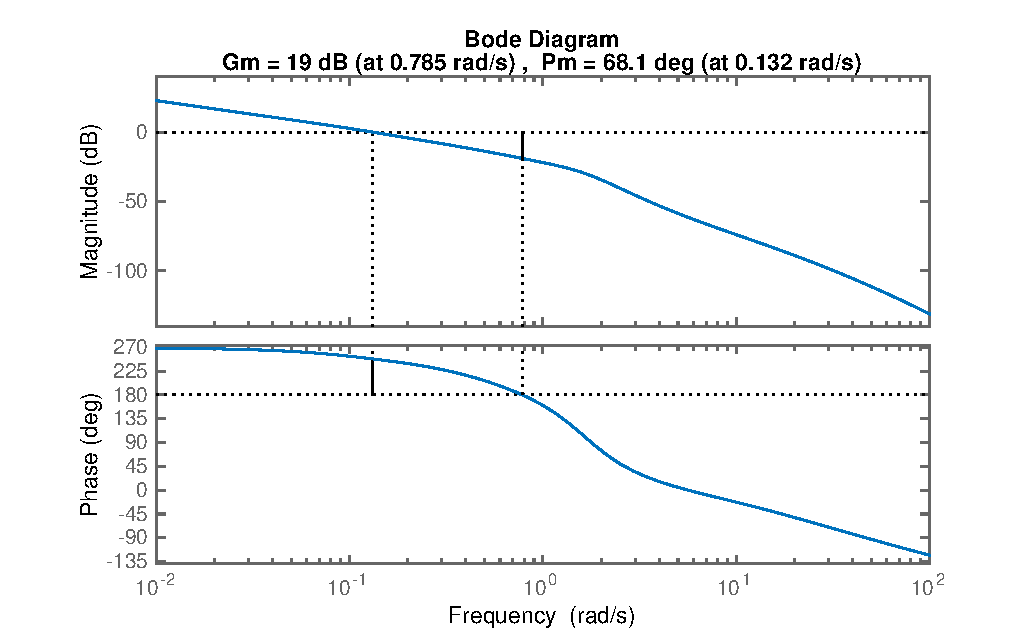
\includegraphics[height=.4\textheight]{figures/open_comp_hdot}
\caption{Open-loop Compensated Bode Diagram for $\dfrac{\dot{h}}{\theta_e}$}
\end{center}
\end{figure}

\begin{figure}[h!]
\begin{center}
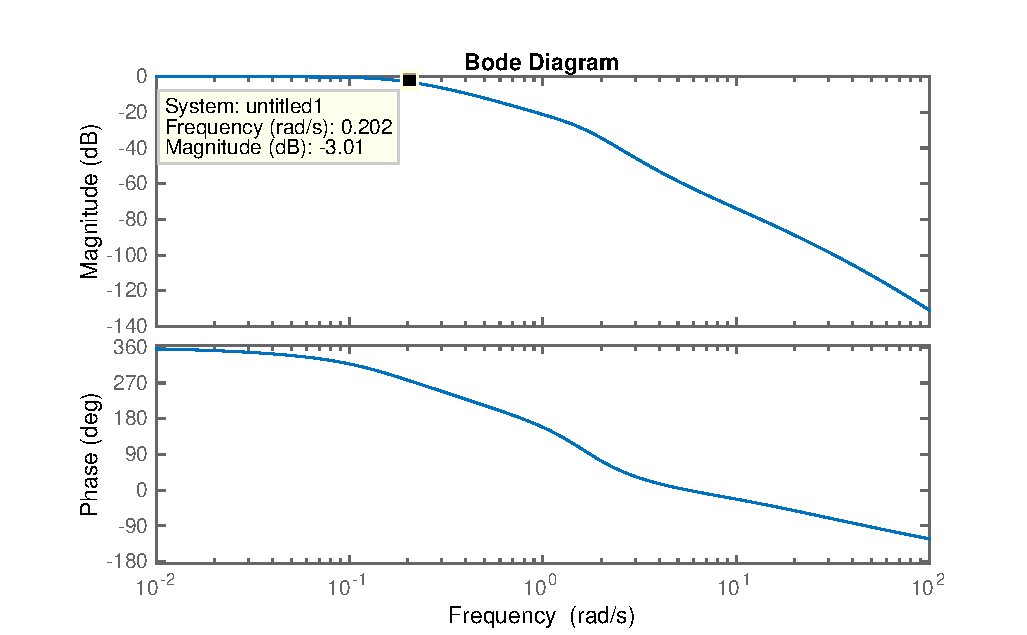
\includegraphics[height=.4\textheight]{figures/close_comp_hdot}
\caption{Close-loop Compensated Bode Diagram for $\dfrac{\dot{h}}{\theta_e}$}
\end{center}
\end{figure}

\clearpage
\section{Response to Inputs}
Two initial conditions were investigated: 
1) a filtered step altitude-rate command of 20 ft/sec and a filtered step airspeed command of 20 ft/sec, applied simultaneously; 
2) a step $u_g$ of 20 ft/sec (a tail wind), without the altitude and airspeed commands. The aircraft reaches steady-state in $\sim50$ sec for both scenarios.

\begin{figure}[h!]
\begin{center}
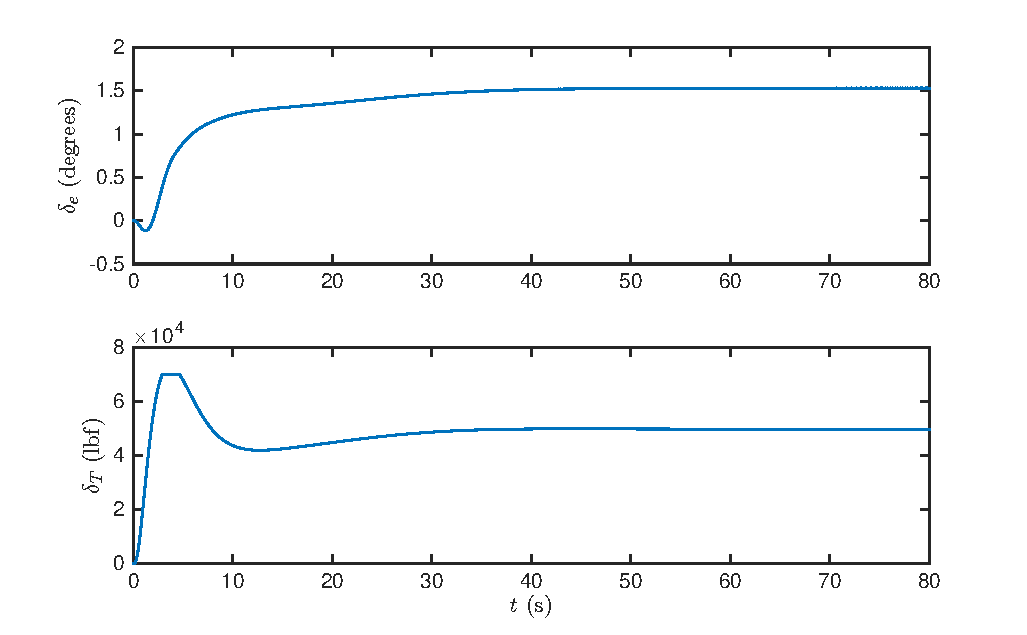
\includegraphics[height=.35\textheight]{figures/inputs1}
\caption{Commanded Inputs for Scenario 1}
\end{center}
\end{figure}

\begin{figure}[h!]
\begin{center}
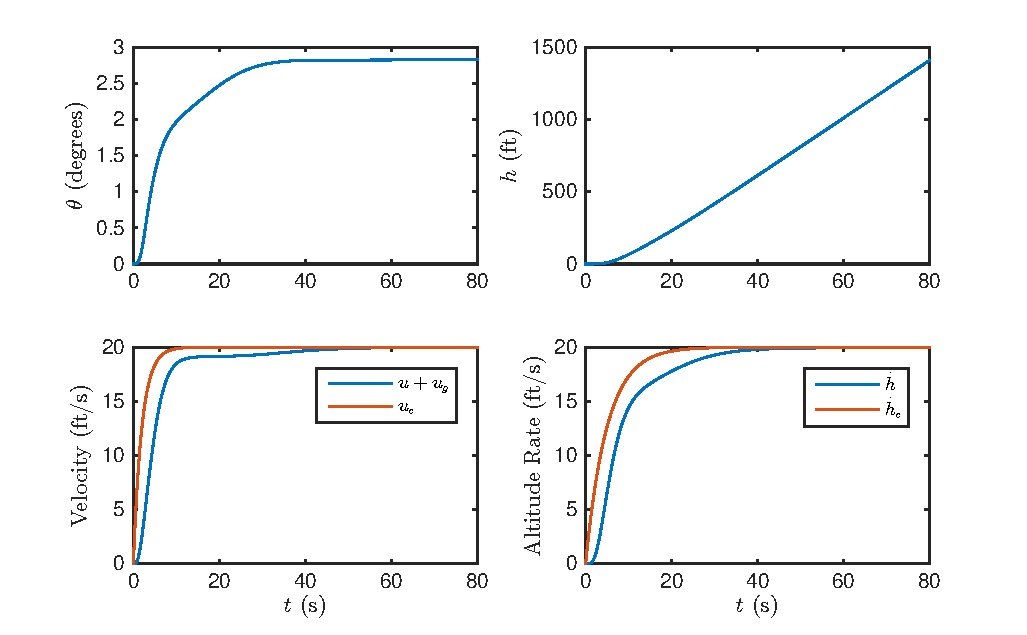
\includegraphics[height=.35\textheight]{figures/outputs2}
\caption{Outputs for Scenario 1}
\end{center}
\end{figure}

\begin{figure}[h!]
\begin{center}
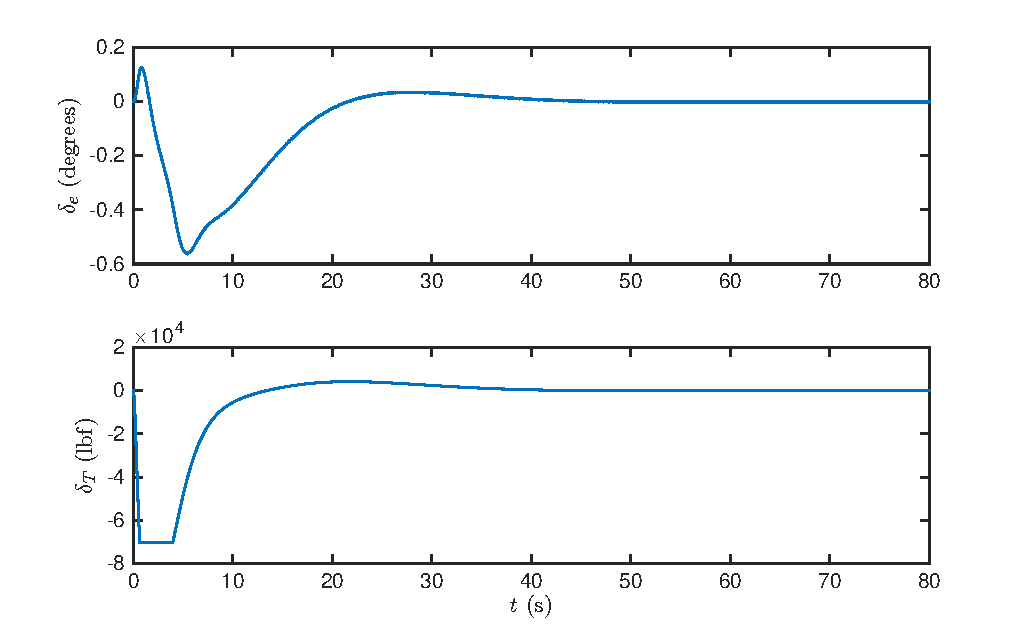
\includegraphics[height=.4\textheight]{figures/inputs3}
\caption{Commanded Inputs for Scenario 2}
\end{center}
\end{figure}

\begin{figure}[h!]
\begin{center}
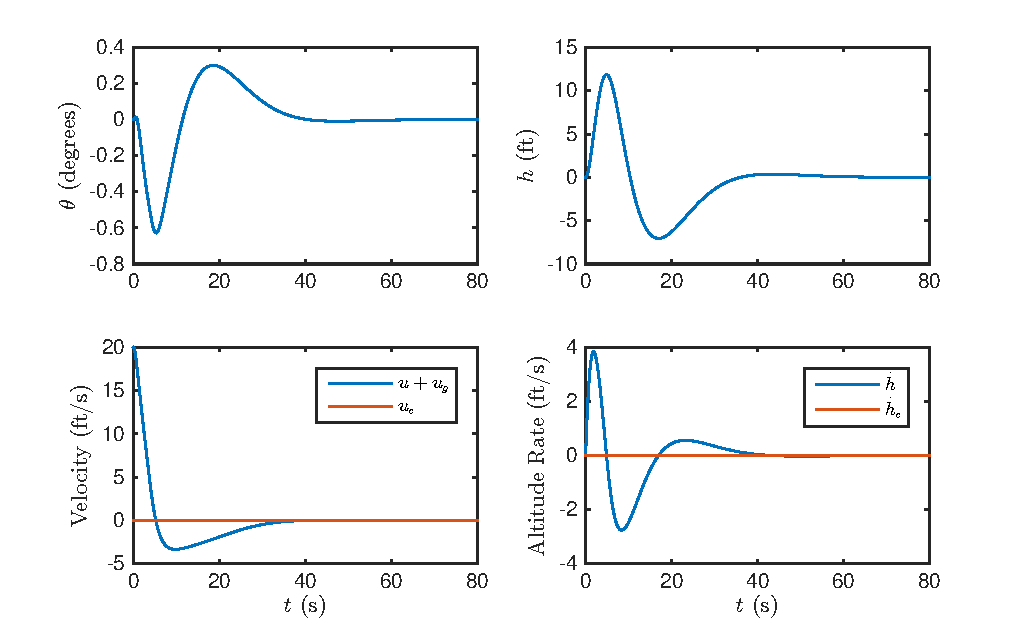
\includegraphics[height=.4\textheight]{figures/outputs4}
\caption{Outputs for Scenario 2}
\end{center}
\end{figure}

\end{document}
